\chapter{Photon energy resolution estimation}\label{sec:appendix_resolution_fits}

Each photon has a true energy, $\EtildeB$, which is the real energy it was produced at (in data) or generated (simulation).
$\tilde{E}_{\gamma}^B$ is not generally the same as the measured energy, commonly denoted as \EB in this thesis.

Based on these two quantities, the resolution of the photon energy measured in the signal-\B meson rest frame is evaluated.
The quantity from \Cref{eq:resolution}:
\begin{equation}
    \EtildeB - \EB
\end{equation}
is fitted with a double-sided Crystal Ball function.
A double-sided Crystal Ball is a generalised version of \Cref{eq:crystal_ball}, where an exponential tail is attached to both sides of the central Gaussian.
This replaced the parameters $\{\alpha,n\}$ with $\{\alpha_L,\alpha_R, n_R, n_L\}$, where indices $R$ and $L$ denote that these parameters represent, correspondingly, `right' or `left' side of the Gaussian.
The main parameter of interest when measuring the resolution is $\sigma$, which corresponds to the width of the central Gaussian and is directly interpreted as the resolution.

The unbinned negative log-likelihood fits are performed in intervals of $\tilde{E}_{\gamma}^B$.
Although all double-sided Crystal Ball parameters are estimated by the fitter, only $\sigma$ is focused on for this study.
The hybrid signal-model samples are fitted, where a good tag-\B meson (based on \Cref{fig:good_tag_definitions}, selected with maximum \feiProb) is used to evaluate the \EB.
For comparison, the same is done where events are only taken if a `perfect' reconstruction of the tag-\B meson is achieved.
The former is visualised in \Cref{fig:resolution_fits}, whereas the latter is in \Cref{fig:issignal_resolution_fits}.
The parameters $\sigma$ and their corresponding uncertainties estimated by the fitter are then summarised in \Cref{fig:resolution_sigmas}.
In \Cref{sec:resolution_studies} further discussion follows.

\begin{figure}[htbp!]
    \centering
    \subcaptionbox{\label{fig:res_1p4}}{
        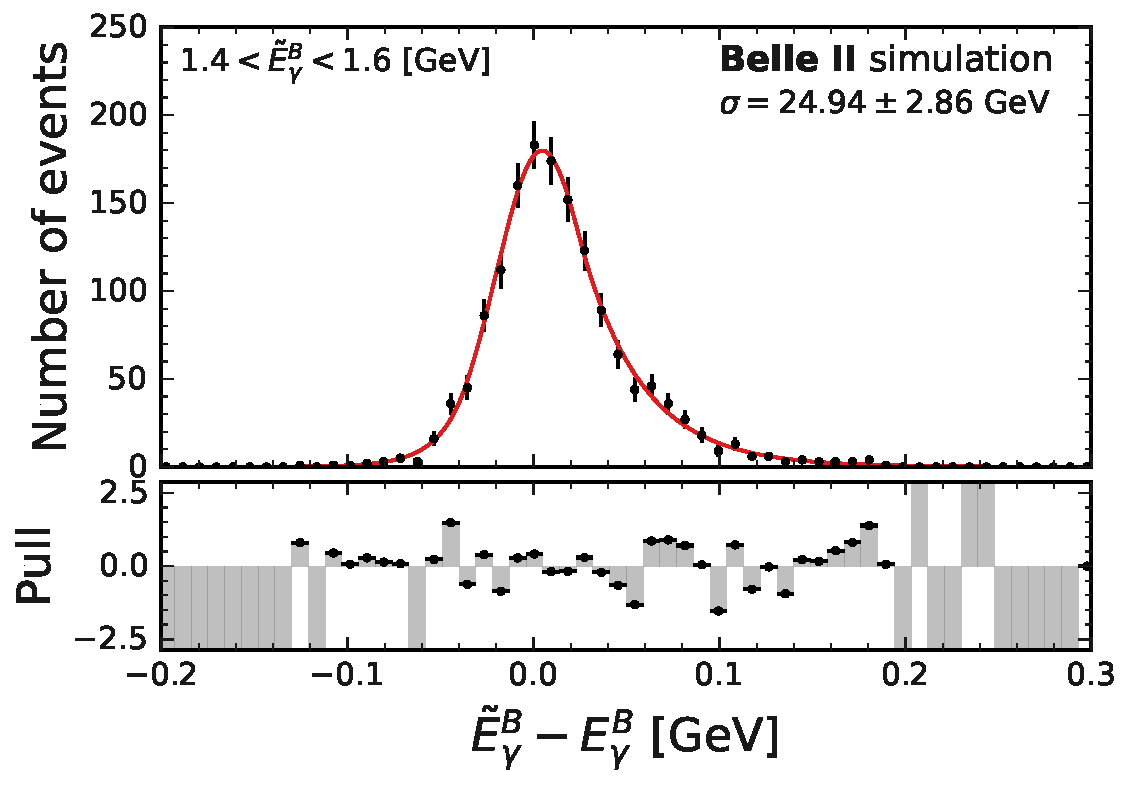
\includegraphics[width=0.31\textwidth]{figures/appendices/resolution_fits/1p4to1p6.pdf}
    }
    \subcaptionbox{\label{fig:res_1p6}}{
        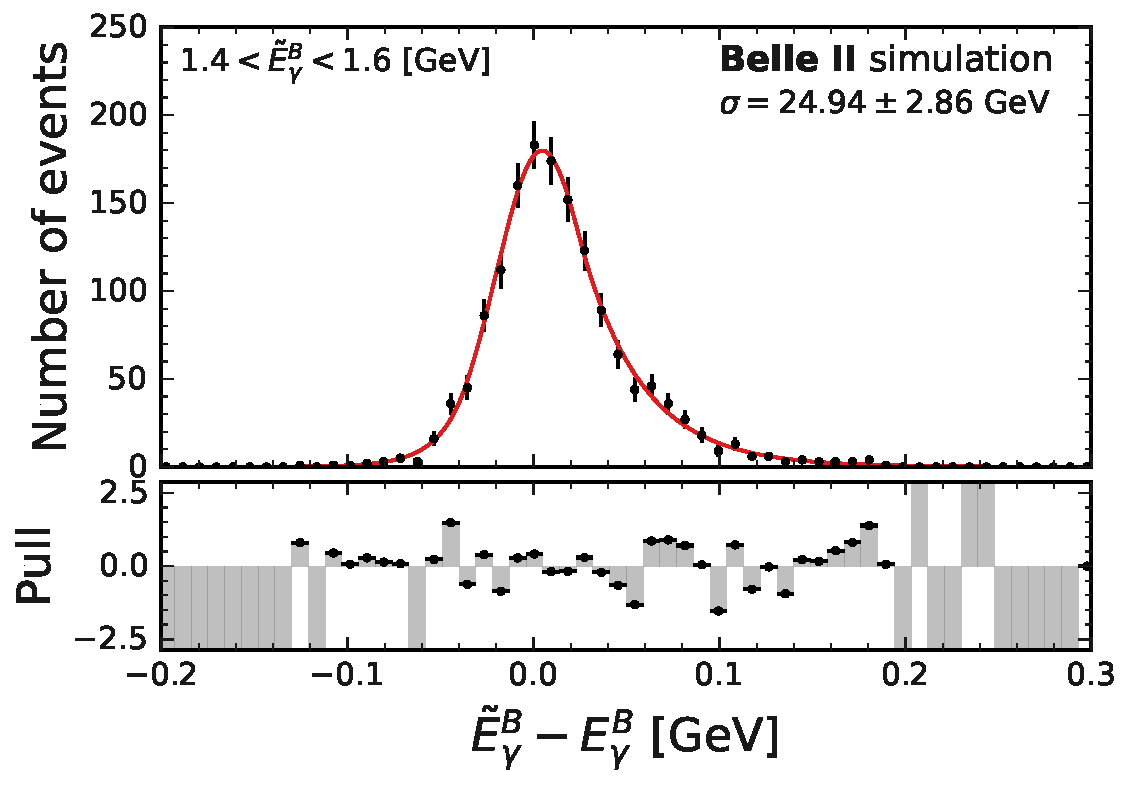
\includegraphics[width=0.31\textwidth]{figures/appendices/resolution_fits/1p4to1p6.pdf}
    }
    \subcaptionbox{\label{fig:res_1p8}}{
        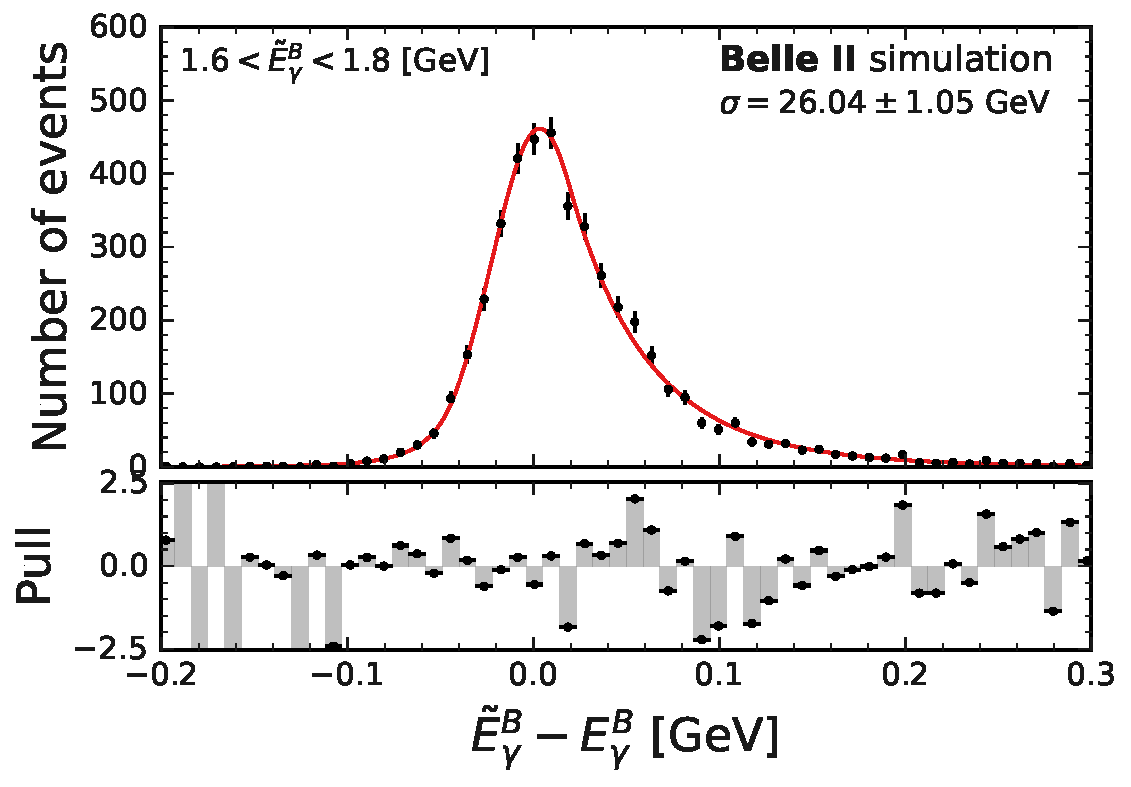
\includegraphics[width=0.31\textwidth]{figures/appendices/resolution_fits/1p6to1p8.pdf}
    }
    \subcaptionbox{\label{fig:res_2p0}}{
        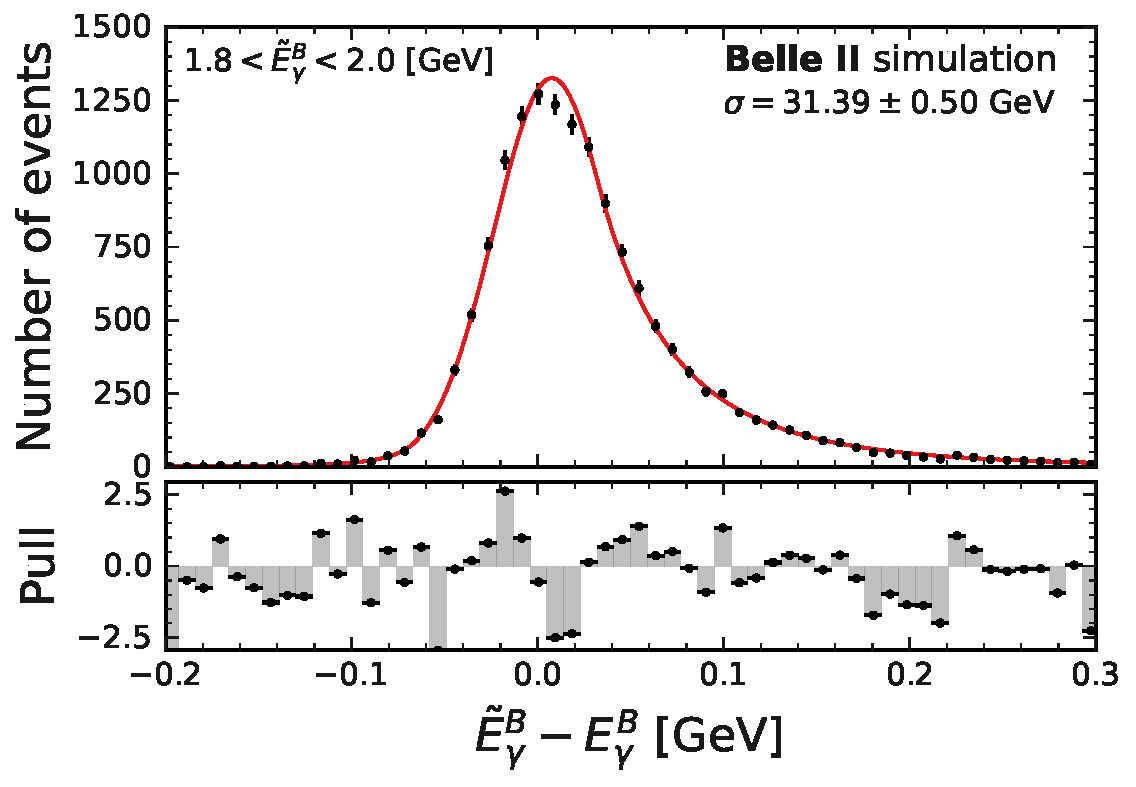
\includegraphics[width=0.31\textwidth]{figures/appendices/resolution_fits/1p8to2p0.pdf}
    }
    \subcaptionbox{\label{fig:res_2p1}}{
        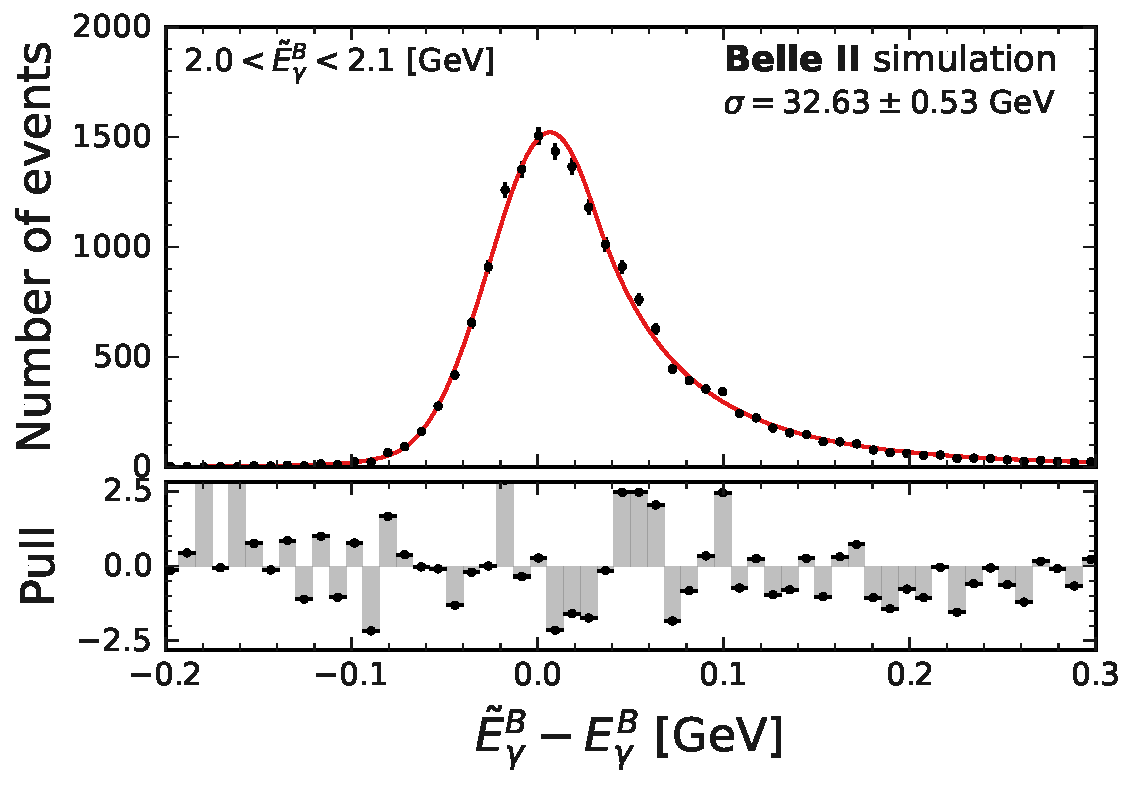
\includegraphics[width=0.31\textwidth]{figures/appendices/resolution_fits/2p0to2p1.pdf}
    }
    \subcaptionbox{\label{fig:res_2p2}}{
        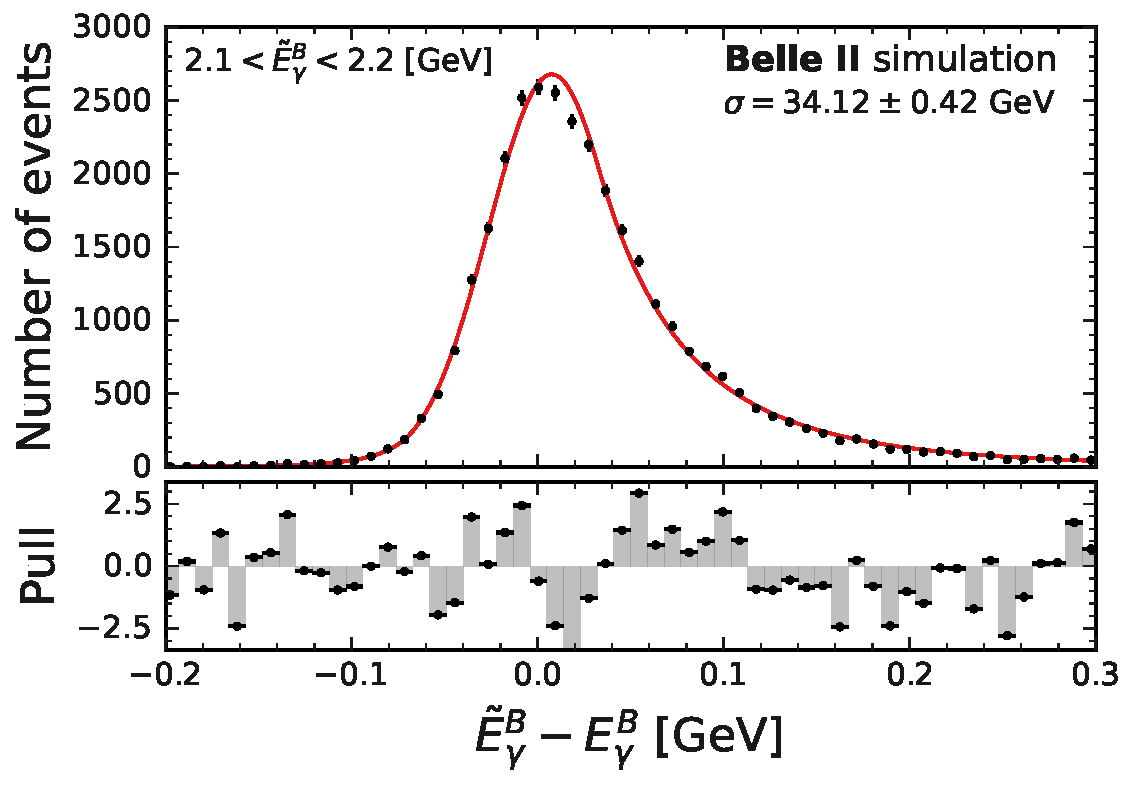
\includegraphics[width=0.31\textwidth]{figures/appendices/resolution_fits/2p1to2p2.pdf}
    }
    \subcaptionbox{\label{fig:res_2p3}}{
        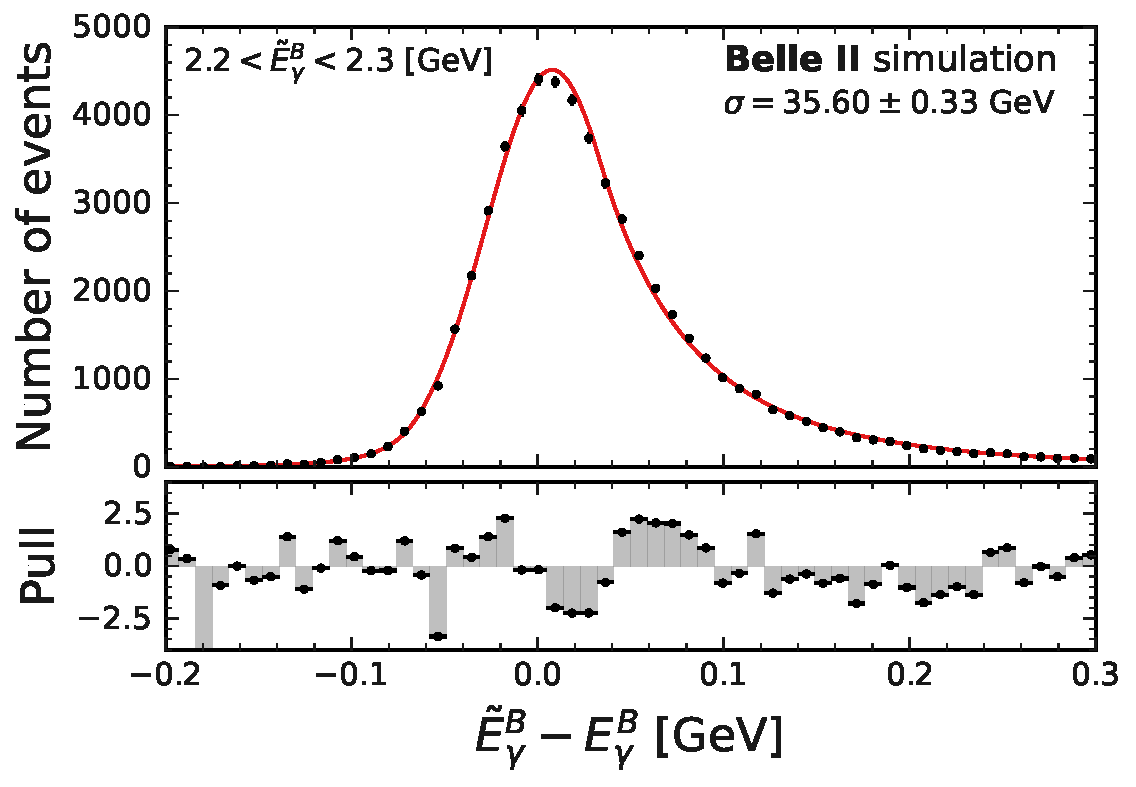
\includegraphics[width=0.31\textwidth]{figures/appendices/resolution_fits/2p2to2p3.pdf}
    }
    \subcaptionbox{\label{fig:res_2p4}}{
        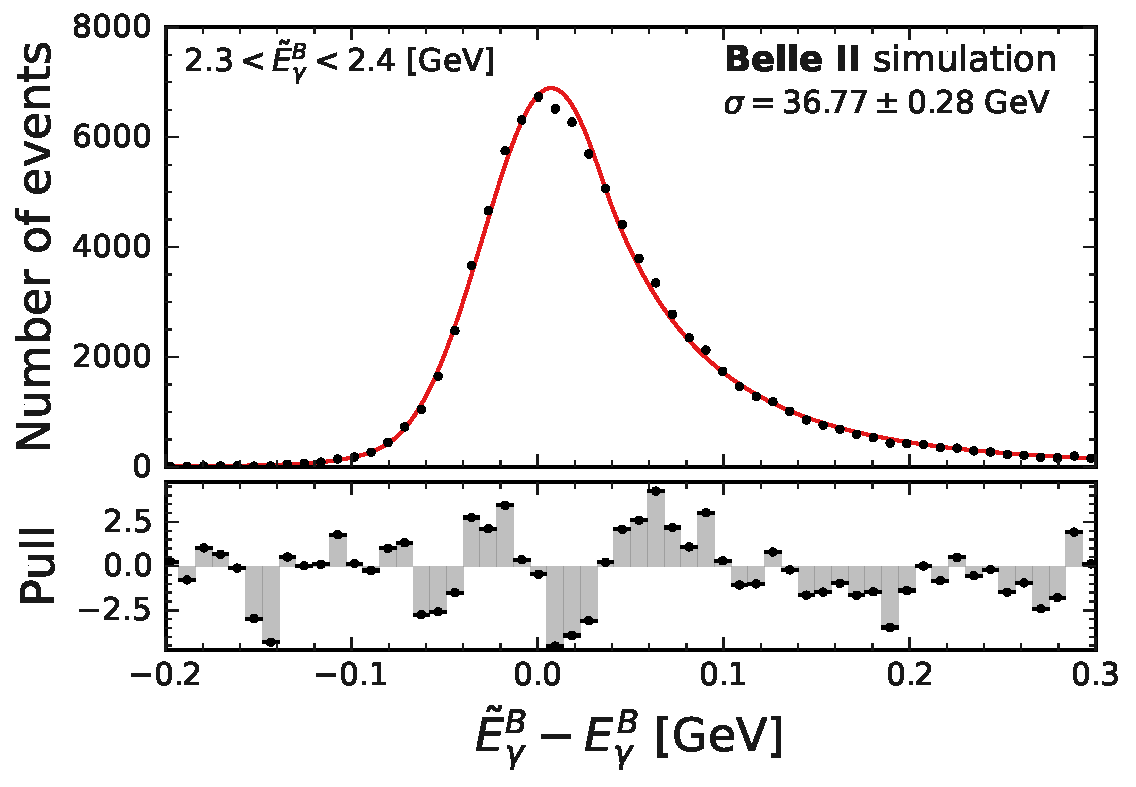
\includegraphics[width=0.31\textwidth]{figures/appendices/resolution_fits/2p3to2p4.pdf}
    }
    \subcaptionbox{\label{fig:res_2p5}}{
        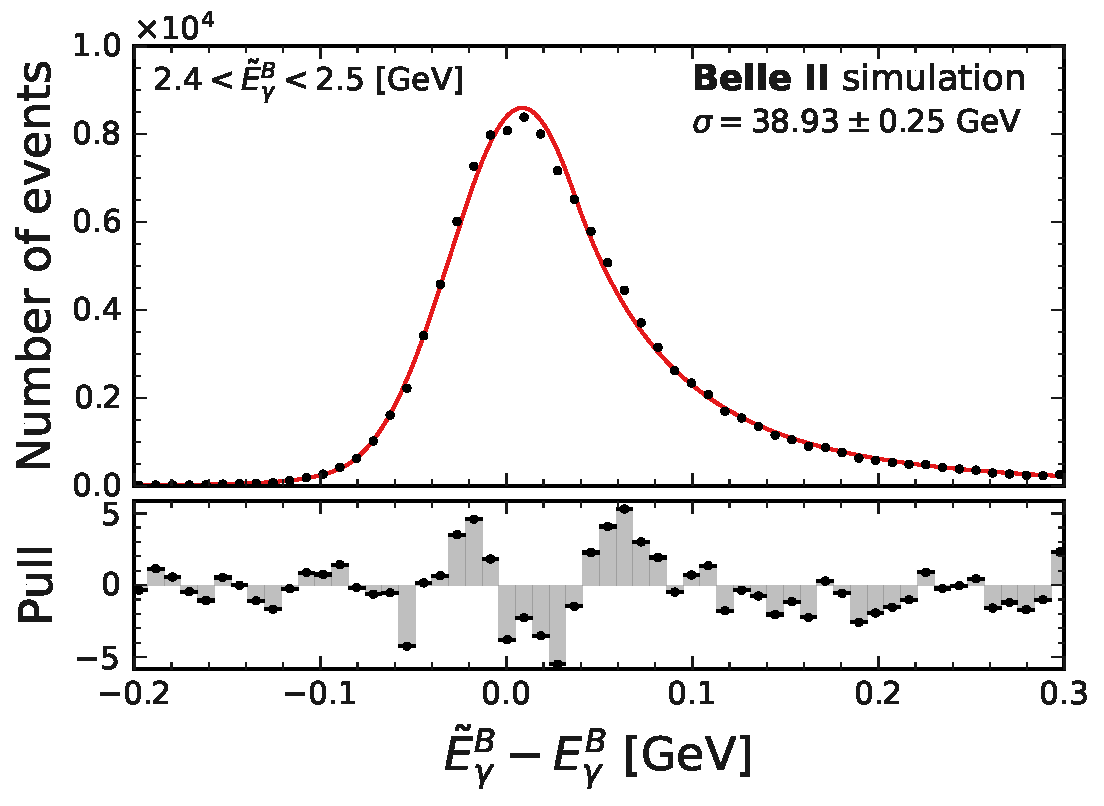
\includegraphics[width=0.31\textwidth]{figures/appendices/resolution_fits/2p4to2p5.pdf}
    }
    \subcaptionbox{\label{fig:res_2p6}}{
        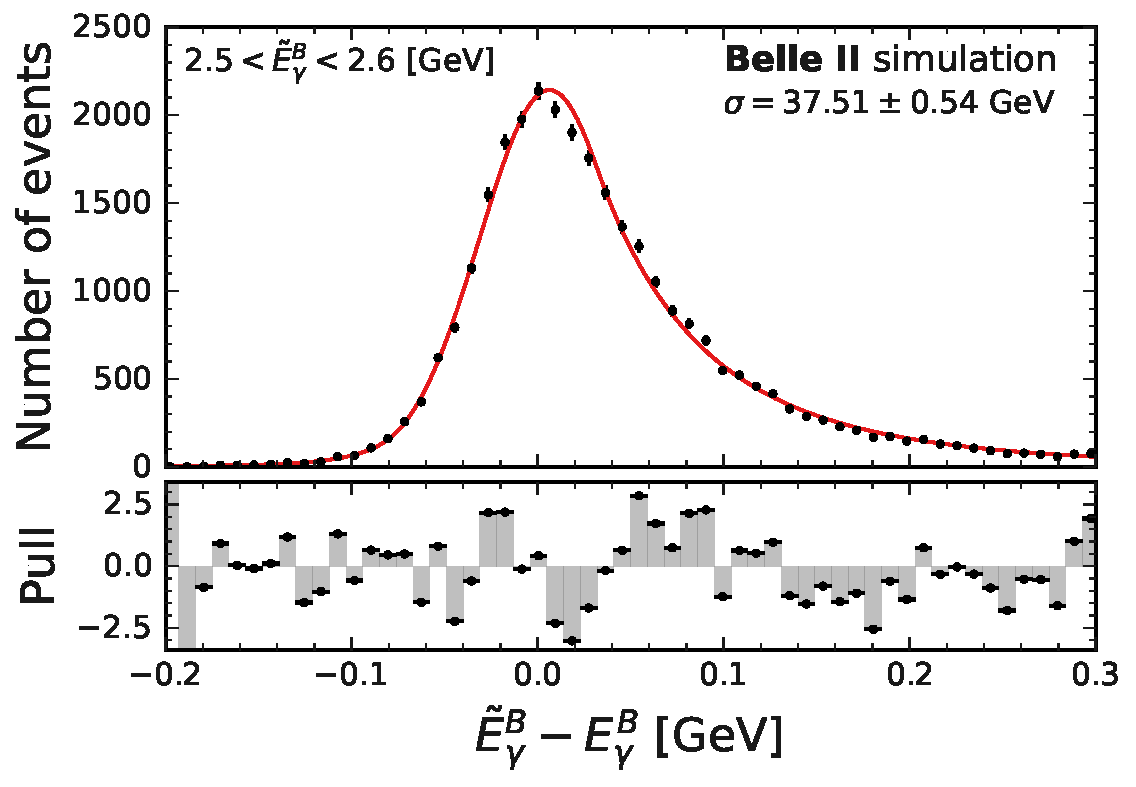
\includegraphics[width=0.31\textwidth]{figures/appendices/resolution_fits/2p5to2p6.pdf}
    }

    \caption{\label{fig:resolution_fits} The double-sided Crystal Ball fits, based on \Cref{eq:resolution},
    on the hybrid signal-model dataset where good tag-\B mesons are used for \EB reconstruction.
    The parameter $\sigma$, corresponding to the width of the central Gaussian part is evaluated.
    This parameter is equated to the resolution of \EB in this analysis.
    The fits are performed in intervals of $\tilde{E}_{\gamma}^B$ and no \BtoXsgamma photons can be produced with $\tilde{E}_{\gamma}^B\gtrsim 2.6~\gev$, due to kinematic constraints.
    }
\end{figure}

\begin{figure}[htbp!]
    \centering
    \subcaptionbox{\label{fig:issignal_res_1p4}}{
        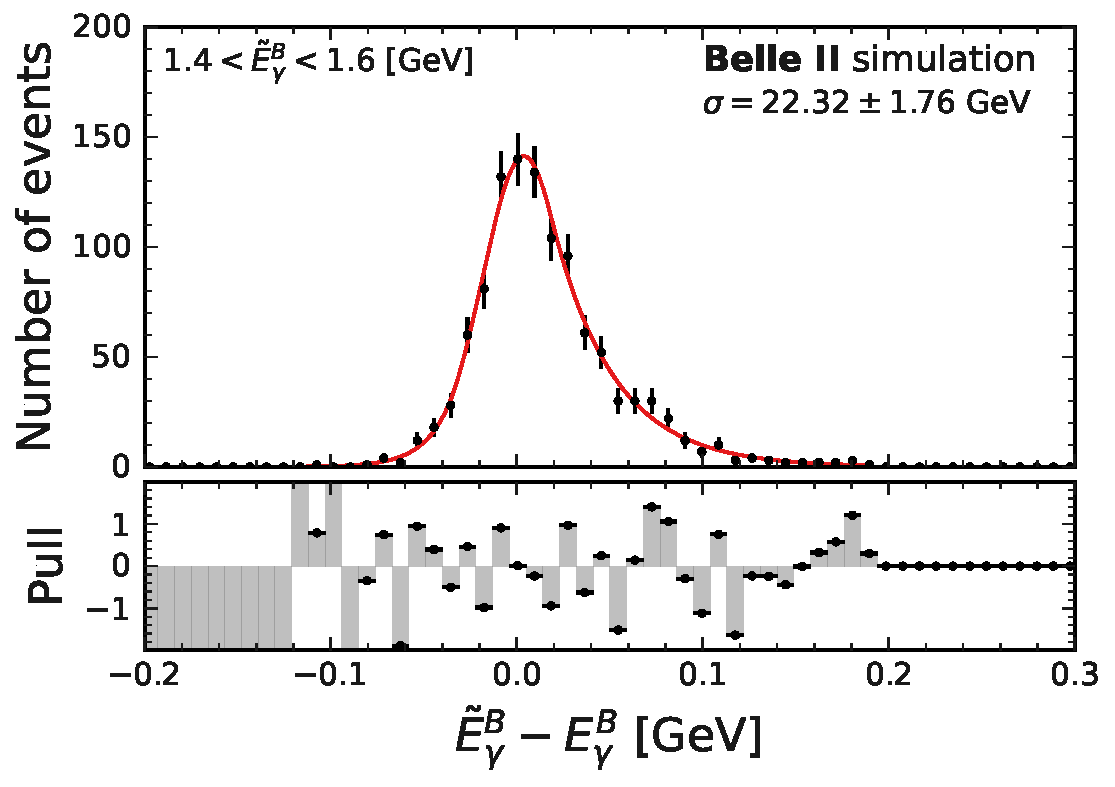
\includegraphics[width=0.31\textwidth]{figures/appendices/resolution_fits/issignal_1p4to1p6.pdf}
    }
    \subcaptionbox{\label{fig:issignal_res_1p6}}{
        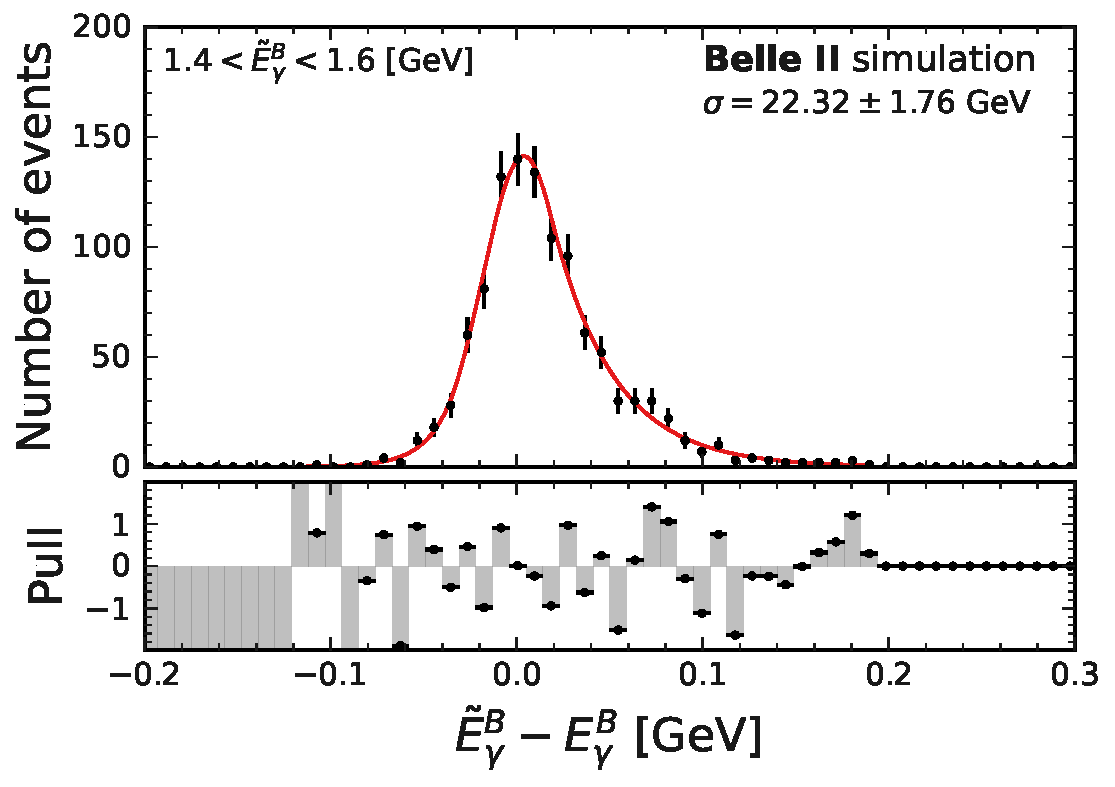
\includegraphics[width=0.31\textwidth]{figures/appendices/resolution_fits/issignal_1p4to1p6.pdf}
    }
    \subcaptionbox{\label{fig:issignal_res_1p8}}{
        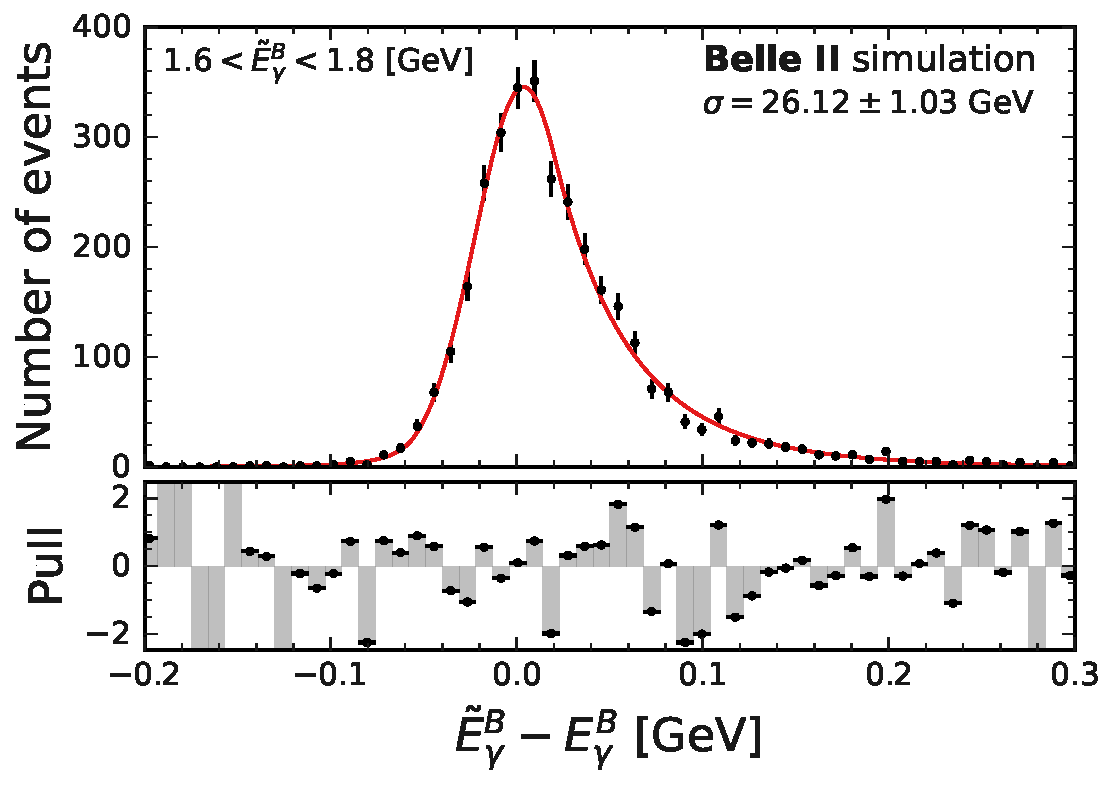
\includegraphics[width=0.31\textwidth]{figures/appendices/resolution_fits/issignal_1p6to1p8.pdf}
    }
    \subcaptionbox{\label{fig:issignal_res_2p0}}{
        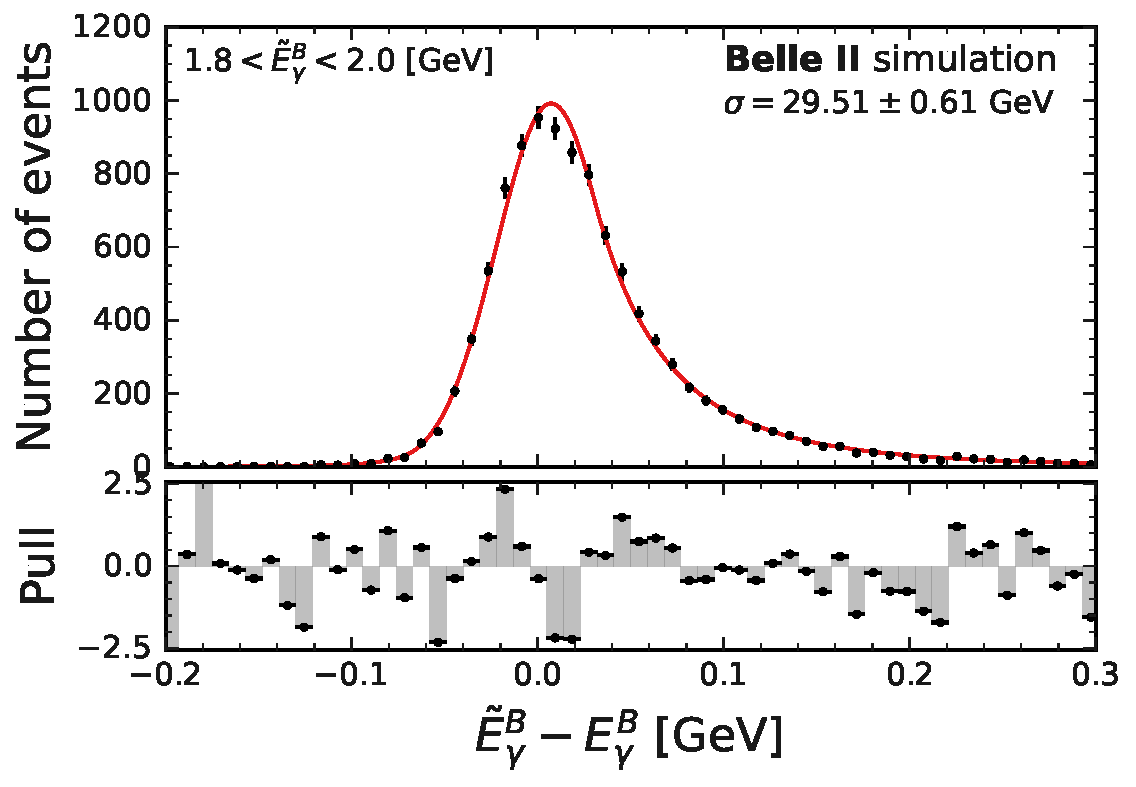
\includegraphics[width=0.31\textwidth]{figures/appendices/resolution_fits/issignal_1p8to2p0.pdf}
    }
    \subcaptionbox{\label{fig:issignal_res_2p1}}{
        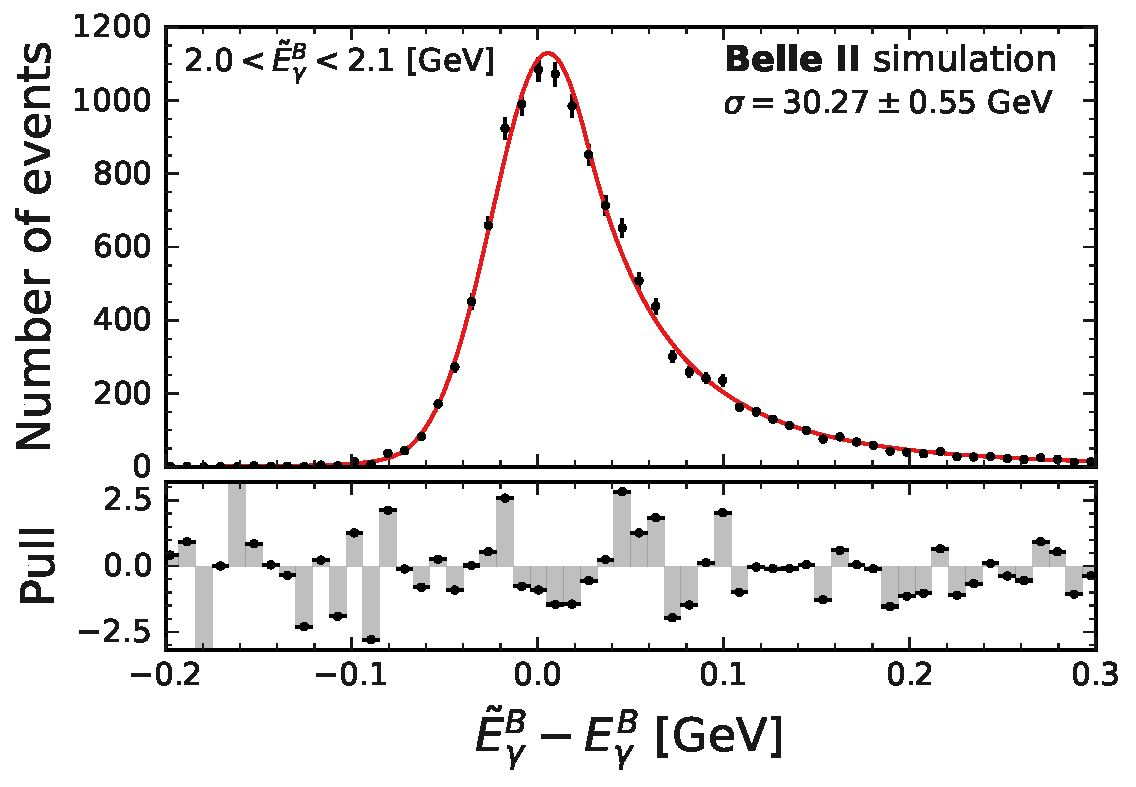
\includegraphics[width=0.31\textwidth]{figures/appendices/resolution_fits/issignal_2p0to2p1.pdf}
    }
    \subcaptionbox{\label{fig:issignal_res_2p2}}{
        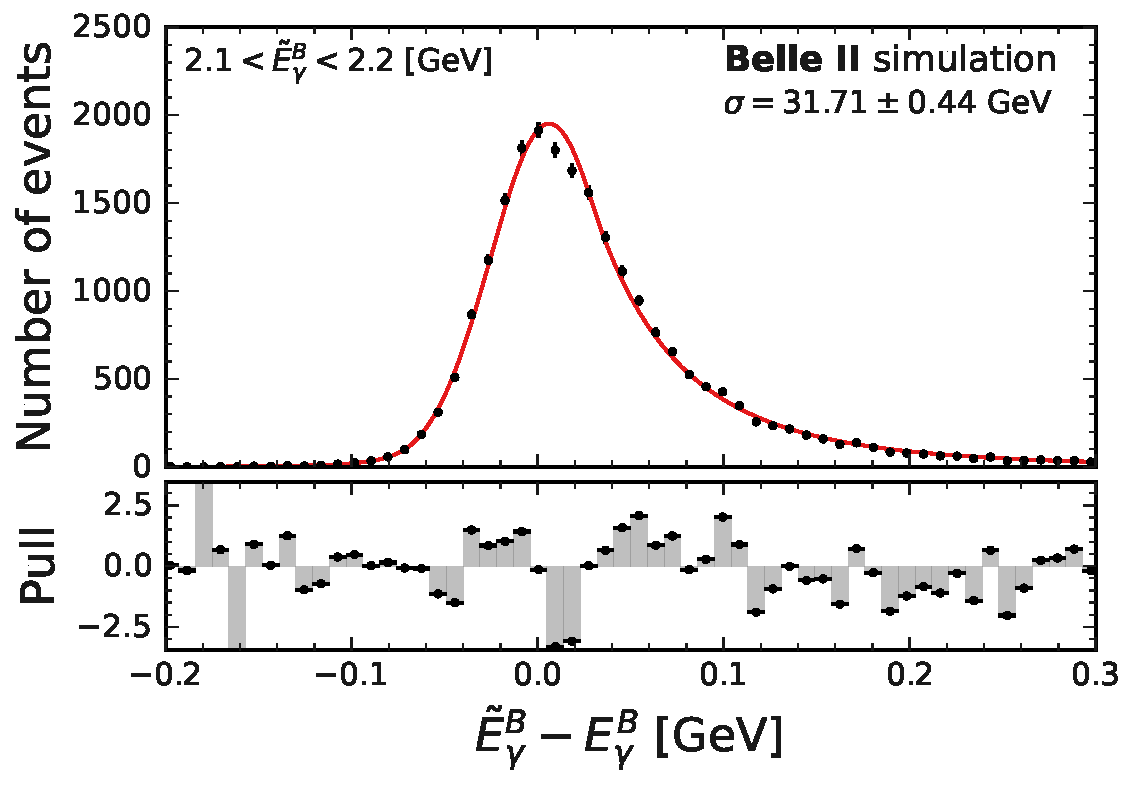
\includegraphics[width=0.31\textwidth]{figures/appendices/resolution_fits/issignal_2p1to2p2.pdf}
    }
    \subcaptionbox{\label{fig:issignal_res_2p3}}{
        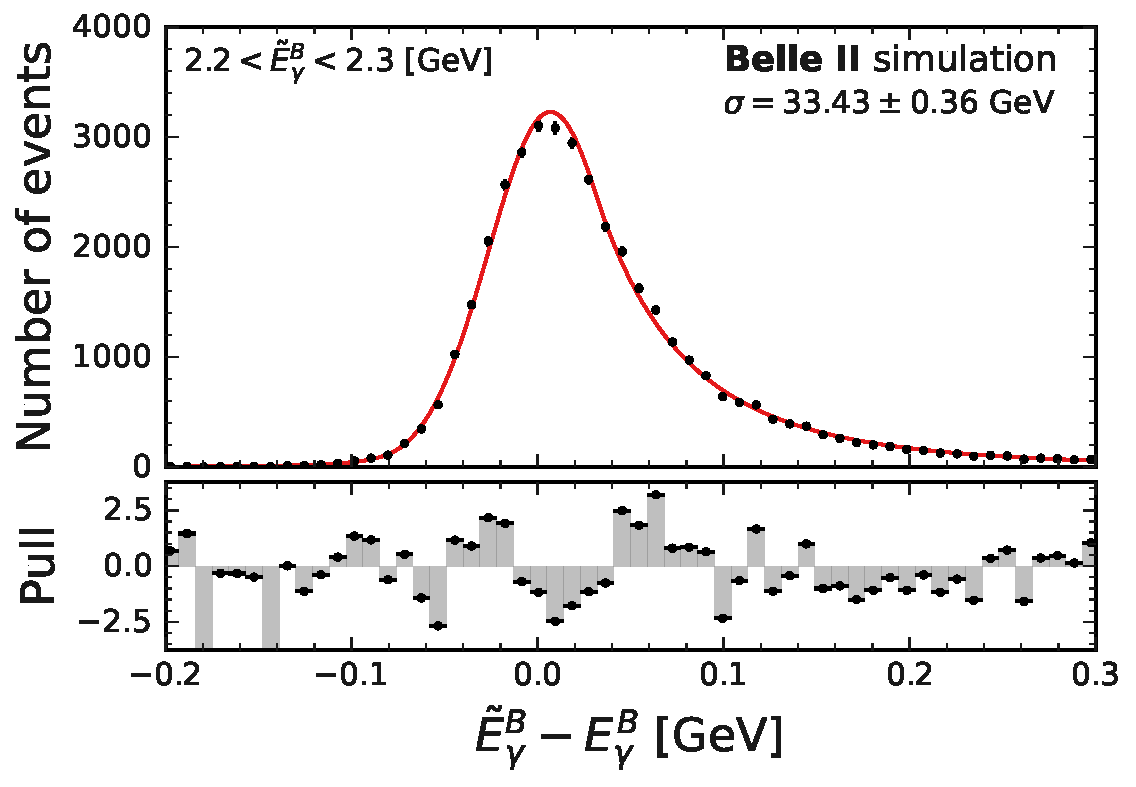
\includegraphics[width=0.31\textwidth]{figures/appendices/resolution_fits/issignal_2p2to2p3.pdf}
    }
    \subcaptionbox{\label{fig:issignal_res_2p4}}{
        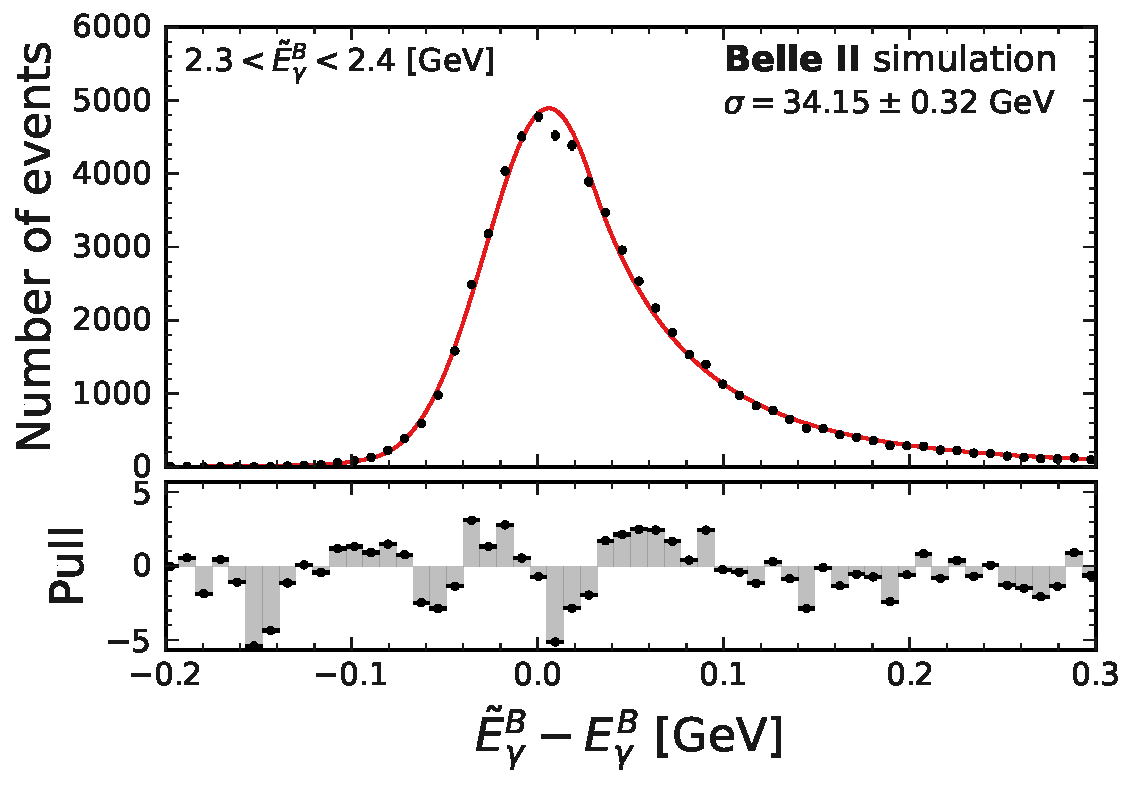
\includegraphics[width=0.31\textwidth]{figures/appendices/resolution_fits/issignal_2p3to2p4.pdf}
    }
    \subcaptionbox{\label{fig:issignal_res_2p5}}{
        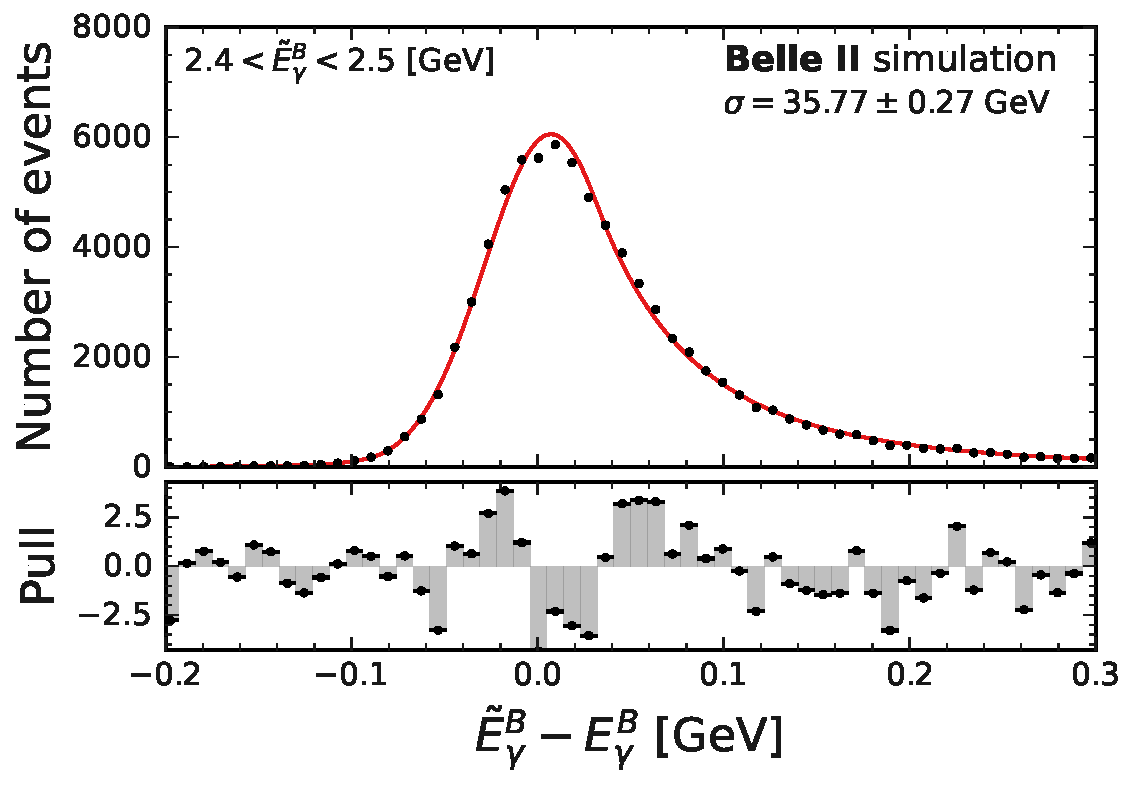
\includegraphics[width=0.31\textwidth]{figures/appendices/resolution_fits/issignal_2p4to2p5.pdf}
    }
    \subcaptionbox{\label{fig:issignal_res_2p6}}{
        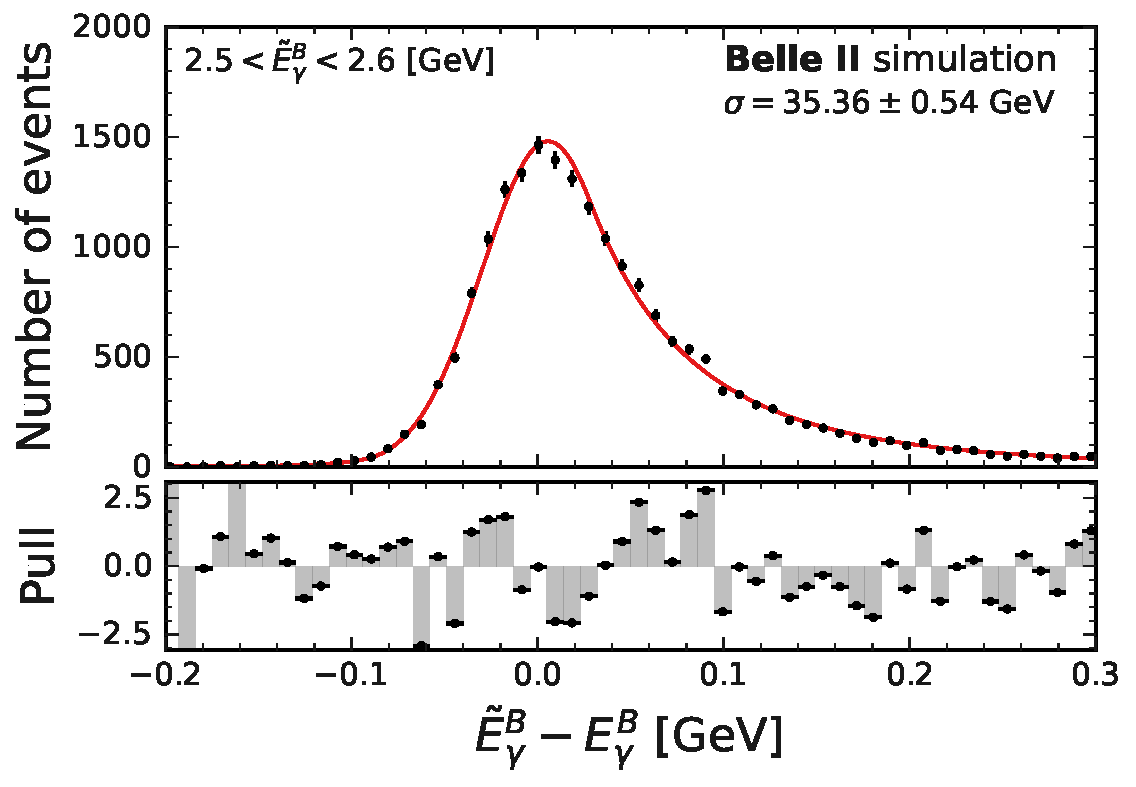
\includegraphics[width=0.31\textwidth]{figures/appendices/resolution_fits/issignal_2p5to2p6.pdf}
    }

    \caption{\label{fig:issignal_resolution_fits} The double-sided Crystal Ball fits, based on \Cref{eq:resolution},
    on the hybrid signal-model dataset where only perfectly reconstructed tag-\B mesons are used for \EB reconstruction.
    The parameter $\sigma$, corresponding to the width of the central Gaussian part is evaluated.
    This parameter is equated to the resolution of \EB in this analysis.
    Note that the fits are performed in intervals of $\tilde{E}_{\gamma}^B$, and no \BtoXsgamma photons can be produced with $\tilde{E}_{\gamma}^B\gtrsim 2.6~\gev$, due to kinematic constraints.
    }
\end{figure}

